\chapter{Local grammars}
\label{chap-grammars}

Local grammars are a powerful tool to represent the majority of linguistic
phenomena. The first section presents the formalism in which these grammars are
represented. Then we will see how to construct and present grammars using Unitex.

\section{The local grammar formalism}
\index{Grammars!formalism}

\subsection{Algebraic grammars}
Unitex grammars are variants of algebraic grammars, also known as context-free
grammars. \index{Grammars!context-free} An algebraic grammar consists of
rewriting rules. Below you see a grammar that matches any number of $a$
characters:

\bigskip $S \rightarrow$ $aS$

$S \rightarrow$ \E

\bigskip
\noindent The symbols to the left of the rules are called \textit{non-terminal
symbols}\index{Symbols!non-terminal}\index{Non-terminal symbols}  since they can
be replaced. Symbols that cannot be replaced by other rules are called
\textit{terminal symbols}\index{Symbols!terminal}. The items at the right side
are sequences of non-terminal and terminal symbols. The epsilon symbol \E ~
designates the empty word. In the grammar above, $S$ is a non-terminal symbol and
$a$ a terminal (symbol). $S$ can be rewritten as either an $a$ followed by a $S$
or as the empty word. The operation of rewriting by applying a rule is called
\textit{derivation}.\index{Derivation} We say that a grammar generates a word if
there exists a sequence of derivations that produces that word. The non-terminal
that is the starting point of the first derivation is called an
\textit{axiom}.\index{Axiom}\index{Rules!rewriting}


\bigskip
\noindent The grammar above also generates the word \textit{aa}, since we can
derive this word according to the axiom $S$ by applying the following derivations:

\bigskip Derivation 1: rewriting the axiom to $aS$

\underline{$S$} $\rightarrow aS$

\bigskip Derivation 2: rewriting $S$ at the right side of $aS$

$S$ $\rightarrow a$\underline{$S$} $\rightarrow aaS$

\bigskip Derivation 3: rewriting $S$ to \E

$S$ $\rightarrow aS \rightarrow aa$\underline{$S$} $\rightarrow aa$

\bigskip
\noindent We call the set of words generated by a grammar the \textit{language
generated by the grammar}. The languages generated by algebraic grammars are
called \textit{algebraic languages}\index{Algebraic languages} or
\textit{context-free languages}\index{Context-free languages}.


\subsection{Extended algebraic grammars}
\index{Grammars!extended algebraic}

Extended algebraic grammars are algebraic grammars where the members on the right
side of the rule are not just sequences of symbols but regular
expressions.\index{Regular expressions} Thus, the grammar that generates a
sequence of an arbitrary number of $a$'s can be written as a grammar consisting
of one rule:

\bigskip $S \rightarrow$ $a^{*}$

\bigskip
\noindent These grammars, also called \textit{recursive transition networks}
(\textit{RTN})\index{Recursive Transition Networks}\index{RTN} or \textit{syntax
diagrams}\index{Syntax diagrams}, are suited for a user-friendly graphical
representation. Indeed, the right member of a rule can be represented as a graph
whose name is the left member of the rule.

\bigskip
\noindent However, Unitex grammars are not exactly extended algebraic grammars, since they
contain the notion of \textit{transduction}.\index{Transduction} This notion,
which is derived from the field of finite state automata, enables a grammar to
produce some output. With an eye towards clarity, we will use the terms grammar
or graph. When a grammar produces outputs, we will use the term
\textit{transducer},\index{Transducer} as an extension of the definition of a
transducer in the area of finite state automata.\index{Automaton!finite state}


\section{Editing graphs}
\label{section-editing-graphs}
\subsection{Creating a graph}
In order to create a graph, click on "New" in the "FSGraph" menu (\ref{fig-fsgraph-menu}).

\begin{figure}[!h]
\begin{center}
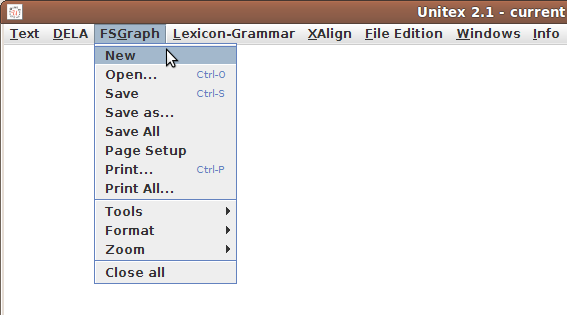
\includegraphics[width=13cm]{resources/img/fig5-1.png}
\caption{FSGraph menu\label{fig-fsgraph-menu}}
\end{center}
\end{figure}

\bigskip
\noindent You will then see the window coming up as in figure~\ref{fig-new-graph}.

\begin{figure}[!h]
\begin{center}
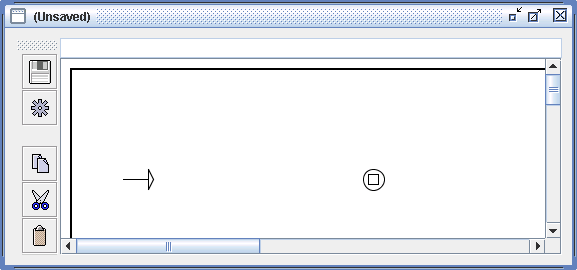
\includegraphics[width=14.5cm]{resources/img/fig5-2.png}
\caption{Empty graph\label{fig-new-graph}}
\end{center}
\end{figure}

\bigskip
\noindent In order to import Intex graphs into Unitex, you have to convert them into Unicode.
The process is the same as for texts (see section~\ref{section-conversion-texte-unicode}).

\bigskip
\noindent The symbol in
arrow form is the \textit{initial state} of the graph.\index{State!initial} The
round symbol with a square is the \textit{final state} of the
graph.\index{State!final} The grammar only recognizes expressions that are
described along the paths between initial and final states.

\bigskip
\noindent In order to create a box, click inside the window while pressing the Ctrl
key.\index{Graph!creating a box}\index{Creating a Box}\index{Boxes!creating}
A blue rectangle will appear that symbolizes the empty box that was created (see
figure~\ref{fig-box-creation}).

\bigskip
\noindent When the box is created, it is automatically selected. 

\begin{figure}[!h]
\begin{center}
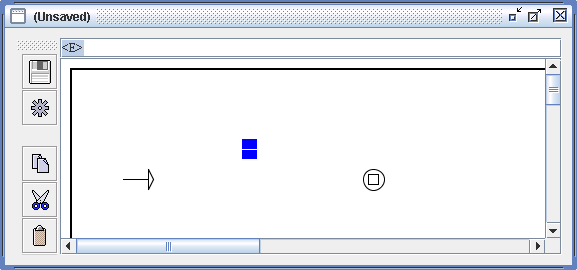
\includegraphics[width=14.5cm]{resources/img/fig5-3.png}
\caption{Creating a box\label{fig-box-creation}}
\end{center}
\end{figure}

\bigskip
\noindent If you use Unitex on a Macintosh device, you must press the "Command key" 
instead of Ctrl in every action involving the Ctrl key.

\bigskip
\noindent You see the contents of the box in the text field at the top of the
window (figure~\ref{fig-box-creation}). The newly created box contains the \verb+<E>+ symbol that represents the empty word
epsilon.\index{\verb+<E>+} Replace this symbol by the text \verb$I+you+he+she+it+we+they$ and
press the Enter key. You see that the box now contains seven lines (see
figure~\ref{fig-pronoun-box}).

\begin{figure}[!h]
\begin{center}
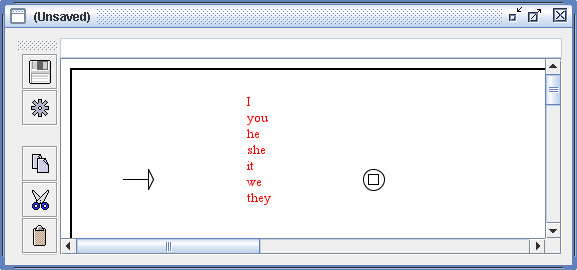
\includegraphics[width=14.5cm]{resources/img/fig5-4.png}
\caption{Box containing
\texttt{I+you+he+she+it+we+they}\label{fig-pronoun-box}}
\end{center}
\end{figure}

\bigskip
\noindent The \verb$+$ character serves as a
separator.\index{\verb$+$} The box is displayed in the form of red text lines since it is 
not connected to another one at the moment.
We often use this type of boxes to insert comments into a
graph. \index{Graph!comments in}\index{Comment!in a graph}

\bigskip
\noindent If you intend to insert comments into a graph, you can create a box starting with \verb$/$.
The text in this box will be displayed in green, and may contain empty lines.
This box can't have any incoming nor outgoing transitions (see
figure~\ref{comment-box}).

\begin{figure}[!h]
\begin{center}
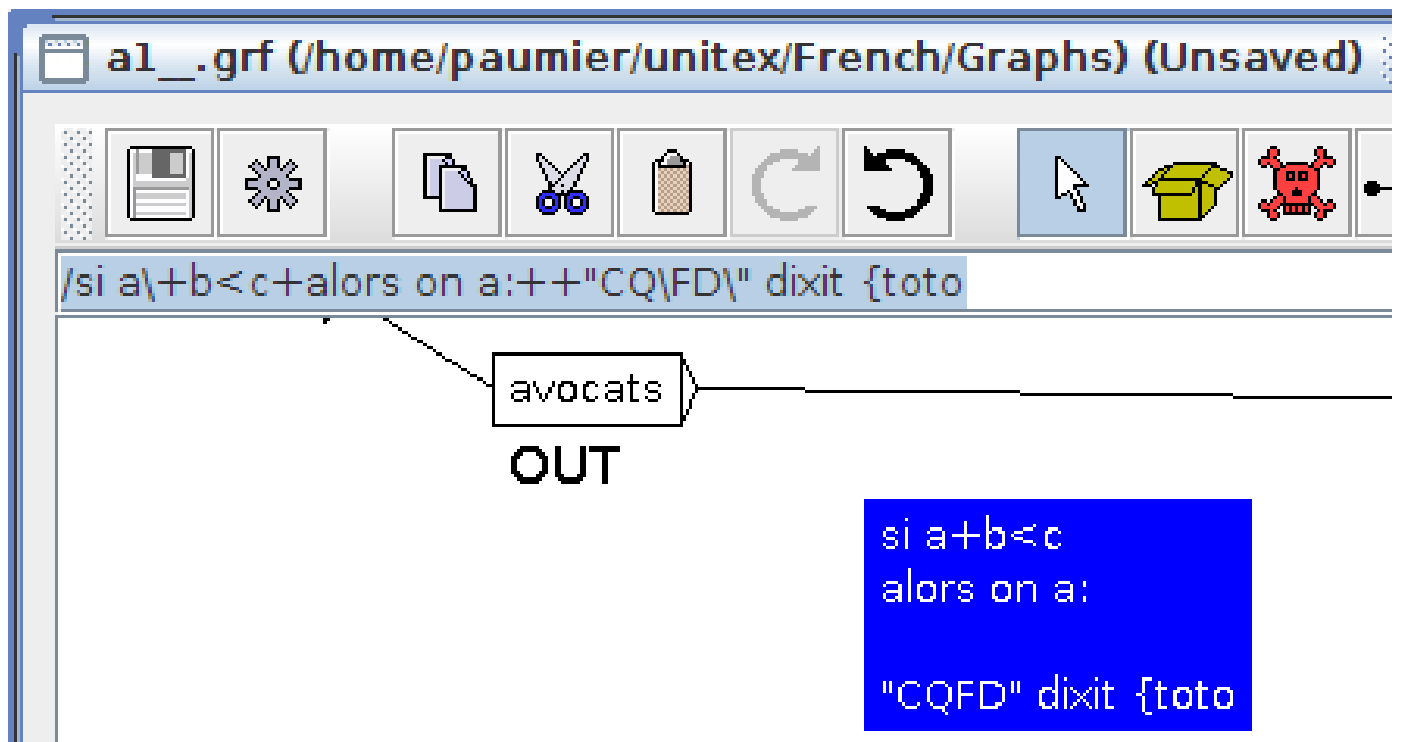
\includegraphics[width=12.5cm]{resources/img/fig5-4b.png}
\caption{Box containing comments\label{comment-box}}
\end{center}
\end{figure}
%\clearpage

\bigskip
\noindent To connect a box to another one, first click on the source box, then
click on the target box.\index{Graph!connecting boxes}\index{Boxes!connecting} If there
already exists a transition between two boxes, it is deleted. It is also possible
to do that by clicking first on the target box and then on the
source box while pressing Shift. In our example, after connecting the box to the initial
and final states of the graph, we get a graph as in
figure~\ref{fig-pronoun-graph}:

\begin{figure}[!ht]
\begin{center}
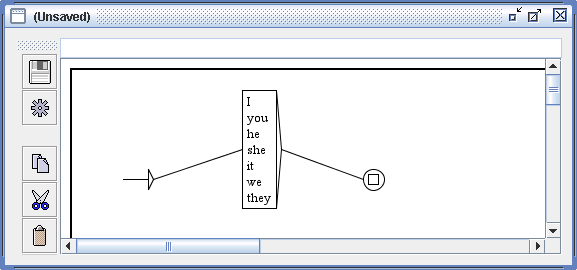
\includegraphics[width=12.5cm]{resources/img/fig5-5.png}
\caption{Graph that recognizes English
pronouns\label{fig-pronoun-graph}}
\end{center}
\end{figure}
%\pagebreak
\bigskip
\noindent NOTE: If you double-click a box, you connect this box to itself (see
figure~\ref{fig-loop-box}). To undo this double-click on the
same box a second time, or use the "Undo" button.

\begin{figure}[!h]
\begin{center}
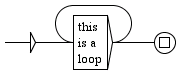
\includegraphics[width=4.5cm]{resources/img/fig5-6.png}
\caption{Box connected to itself\label{fig-loop-box}}
\end{center}
\end{figure}

\bigskip
\noindent Click on "Save as..." in the "FSGraph" menu to save the graph.
\index{Graph!saving} By default, Unitex proposes to save the graph in the
sub-directory \verb+Graphs+ in your personal folder. You can see if the 
graph was modified after the last
saving by checking if the title contains the text \verb+(Unsaved)+.

\bigskip
\noindent Loops are allowed in graphs. They can be around a single box, as in fig.~\ref{fig-loop-box},
or around several boxes, as in fig.~\ref{multi-selection}.
The content of the loop will be recognized any number of times in sequence.
You can set limits to the number of times, but only for a loop around a single box:
see section~\ref{nb-repetitions}.

\bigskip
\noindent When editing a graph you can bring up a specific contextual menu ( fig.~\ref{contextual-menu}) to 
perform standard graph edition operations by right clicking in the background of the graph window.

\bigskip
\begin{figure}[!h]
\begin{center}
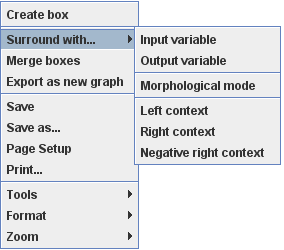
\includegraphics[width=7.5cm]{resources/img/fig5-6b.png}
\caption{contextual menu\label{contextual-menu}}
\end{center}
\end{figure}

\noindent This menu will offer several operations that are frequently used when editing a graph.
\begin{itemize}
\item create a new box
\item save, print the current graph or set up the page parameters
\item the usual "Tools", "Format" and "Zoom" menu also accessible in the FSGraph menu 
\end{itemize}
If one or several boxes are currently selected, the following menus will be accessible, allowing you to apply specific operations to these sets of boxes. Otherwise, these menus are useless and therefore non accessible. 
\begin{itemize}
\item surround selected boxes with an input or output variable definition, with contexts, or with Morphological mode delimiters. These operations are also accessible via the Toolbar of the graph edition window (see section~\ref{toolbar-commands}). 
\item merge selected boxes
\item export as a new graph
\end{itemize}
\bigskip


\subsection{Sub-Graphs}
\label{section-subgraphs}
\index{Graph!calling a sub-graph}\index{\verb+:+}
In order to call a sub-graph, its name is inserted into a box and preceded by the
\verb+:+ character. If you enter the text:

\bigskip
\verb$alpha+:beta+gamma+:E:\greek\delta.grf$

\bigskip
\noindent into a box, you get a box similar to the one in
figure~\ref{fig-subgraph-call}:

\medskip
\begin{figure}[h]
\begin{center}
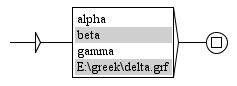
\includegraphics[width=6cm]{resources/img/fig5-7.png}
\caption{Graph that calls sub-graphs \texttt{beta} and
\texttt{delta}\label{fig-subgraph-call}}
\end{center}
\end{figure}

\noindent You can indicate the full name of the graph
(\verb$E:\greek\delta.grf$) or simply the base name without the path (\verb$beta$); 
in this case, the sub-graph is expected to be in the same directory as the graph that references
it. References to absolute path names should as a rule be avoided, since such
calls are not portable. If you use such an absolute path name, the graph compiler
will emit a warning (see figure~\ref{fig-warning-absolute-graph-name}).

\begin{figure}[!h]
\begin{center}
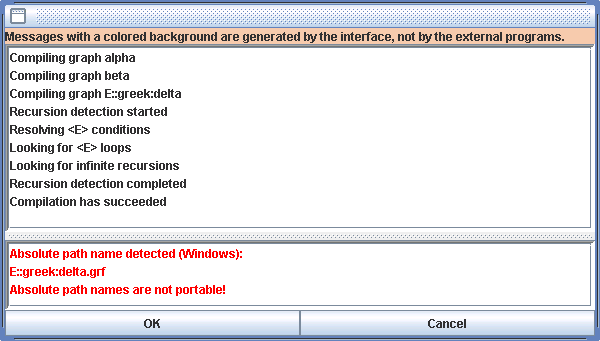
\includegraphics[width=14.5cm]{resources/img/fig5-8.png}
\caption{Warning about a non portable graph
name\label{fig-warning-absolute-graph-name}}
\end{center}
\end{figure}


\bigskip
\noindent For portability you should not use \verb+\+ or \verb+/+ as separator
in graph path names. Use instead \verb+:+ which is understood as a
system-independent separator. In figure~\ref{fig-warning-absolute-graph-name}
\verb+\+ and \verb+/+ are internally converted by the graph compiler to \verb+:+
(\verb+E::greek:delta.grf+).


%\clearpage
%\bigskip

\bigskip
\noindent \textbf{Graph repository}
\label{section-repository}

\bigskip
\noindent When you need to call a grammar $X$ inside a grammar $Y$, a simple
method is to copy all the graphs of $X$ into the directory that contains the
graphs of $Y$. This method raises two problems:

\begin{itemize}
  \item the number of graphs in the directory grows quickly;
  \item two graphs cannot share the same name.
\end{itemize}

\noindent To avoid that, you can store the grammar $X$ in a special directory,
called the \textit{graph repository}.\index{Graph!repository} This directory is a
kind of library where you can store graphs, and then call them using \verb+::+
instead of \verb+:+. To use this mechanism, you first need to set the path to the
graph repository. Go into the "Info>Preferences...>Directories" menu, and select
your directory in the "Graph repository" frame (see Figure \ref{directories}).
There is one graph repository per language, so feel free to share or not the same
directory for all the languages you work with.

\begin{figure}[!h]
\begin{center}
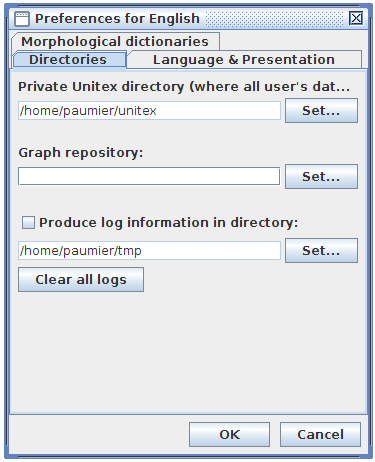
\includegraphics[width=8cm]{resources/img/fig5-10.png}
\caption{Setting the path to the graph repository\label{directories}}
\end{center}
\end{figure}

%\clearpage

\bigskip
\noindent Let us assume that we have a repository tree as on Figure
\ref{repository}. If we want to call the graph named \verb+DET+ that is located
in sub-directory \verb+Johnson+, we must use the call

% do not remove this line jump
\noindent \verb+::Det:Johnson:DET+
(see Figure \ref{repository-graph-call}\,\footnote{To avoid confusion, graph calls
that refer to the repository are displayed in brown instead of grey.}).


\bigskip
\begin{figure}[!h]
\begin{center}
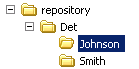
\includegraphics[width=3.9cm]{resources/img/fig5-11.png}
\caption{Graph repository example\label{repository}}
\end{center}
\end{figure}

\begin{figure}[!h]
\begin{center}
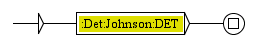
\includegraphics[width=6.7cm]{resources/img/fig5-12.png}
\caption{Call to a graph located in the
repository\label{repository-graph-call}}
\end{center}
\end{figure}

%\clearpage

\noindent TRICK: If you want to avoid long path names like
\verb+::Det:Johnson:DET+, you can create a graph named \verb+DET+ and put it the
repository root (here \verb+D:\repository\DET.grf+). In this graph, just put a
call to \verb+::Det:Johnson:DET+. Then, you can just call \verb+::DET+ in your
own graphs. This has two advantages: 1) you do not have long path names; 2) you
can modify the graphs in your repository with no constraint on your own graphs,
because the only graph that will have to be modified is the one located at the
repository root.

\begin{figure}[h!]
\begin{center}
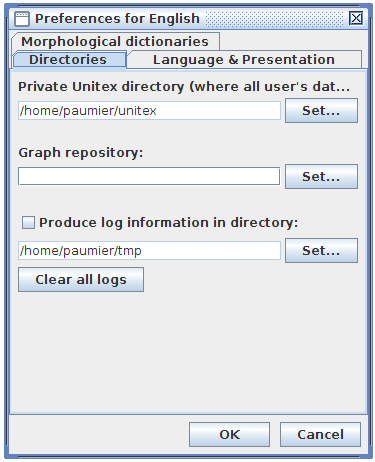
\includegraphics[width=7cm]{resources/img/fig5-9.png}
\caption{Missing called sub-graphs appear in red\label{call-colours}}
\end{center}
\end{figure}


\bigskip
\noindent Calls to sub-graphs are represented in the boxes by grey lines, as in Fig.~\ref{call-colours}, or brown
lines in the case of graphs located in the repository, as in Fig.~\ref{repository-graph-call}. If the .GRF File of the sub-graph is not found at the path you indicated, Unitex will try to find a fst2 file of the same name. If Unitex can't find any of the .grf and .fst2 files, the call to the missing subgraph will be displayed on a red line. 
On Windows, you can open a sub-graph by clicking on the grey line while pressing the Alt key.
On Linux, the <Alt+Click>  combination is intercepted by the system:\footnote{If you are 
working on KDE, you can deactivate <Alt+Click> in kcontrol.} in order to open a
sub-graph, middle-click on its name, or click on its name by pressing the left and the right mouse buttons
simultaneously.

\bigskip
\noindent The list of subgraphs called from the current graph and the graphs in which the current graph is called can be displayed by clicking on the second and third button of the fourth set of buttons in the toolbar command (see Figure~\ref{list-called-graphs} and
Figure~\ref{fig-toolbar} in section~\ref{toolbar-commands}).
In these Lists of subgraphs : 
\begin{itemize}
\item sub-graphs directly called from the current graph appear with their simple filename
\item sub-graphs indirectly called from one of the graphs called by the current graph appear with an arrow before their filename.
\item sub-graphs that appear in one of the graphs that are called from the current one but that are unplugged and never processed appear in orange
\item sub-graphs that are not found (neither .grf nor .fst2) appear in red
\end{itemize}

\begin{figure}[!h]
\begin{center}
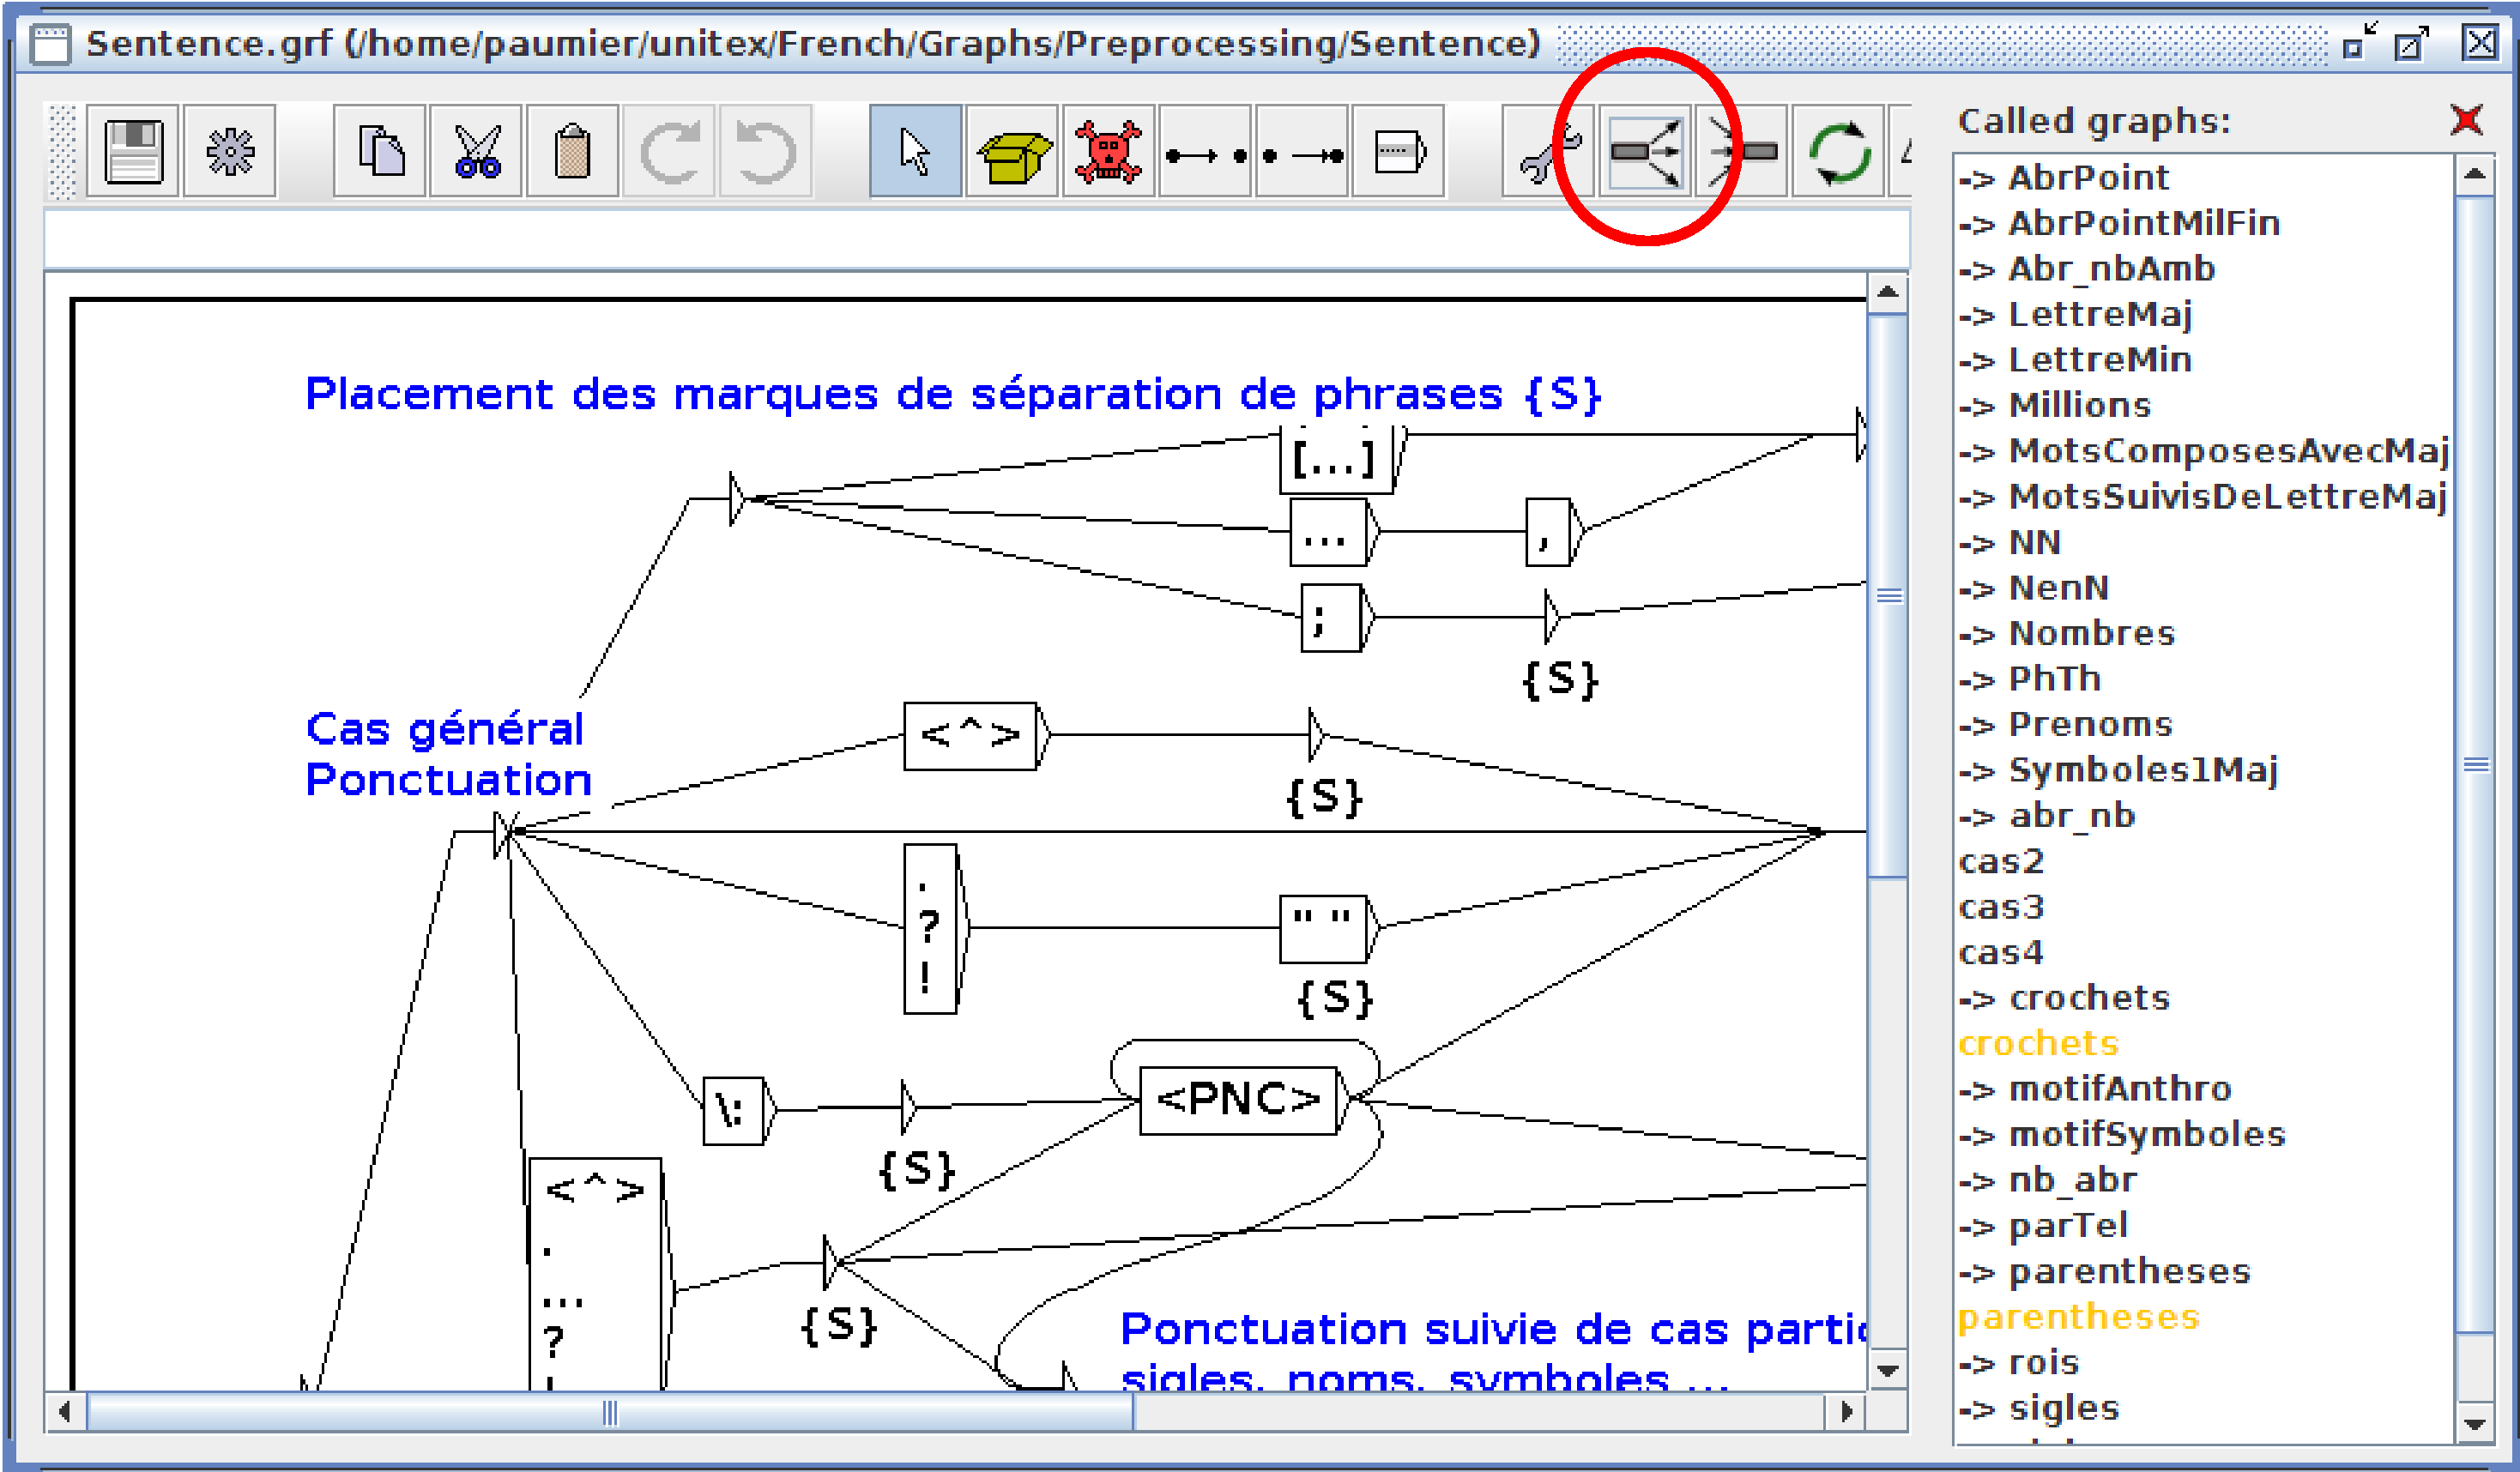
\includegraphics[width=15.2cm]{resources/img/fig5-12b.png}
\caption{Display the list of all called graphs\label{list-called-graphs}}
\end{center}
\end{figure}

\subsection{Manipulating boxes}
\index{Multiple selection}\index{Boxes!selection}

You can select several boxes using the mouse. In order to do so, click and drag the
mouse without releasing the button. When you release the button, all boxes
touched by the selection rectangle will be selected and are displayed in
white on a blue background, as shown on Figure \ref{multi-selection}.

\begin{figure}[!ht]
\begin{center}
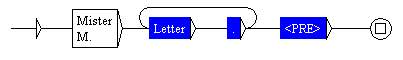
\includegraphics[width=10cm]{resources/img/fig5-13.png}
\caption{Selecting several boxes\label{multi-selection}}
\end{center}
\end{figure}
%\bigskip
\noindent You can select several boxes by keeping simultaneously the <CTRL> and <SHIFT> keys pressed and by clicking on every box you want to add to your current selection. This way you can select several boxes without selecting all the boxes located in their area.

\begin{figure}[!ht]
\begin{center}
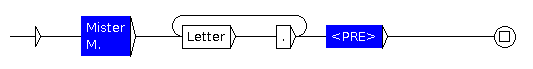
\includegraphics[width=10cm]{resources/img/fig5-13b.png}
\caption{Selecting distant boxes\label{multi-selection}}
\end{center}
\end{figure}
\bigskip
\noindent When boxes are selected, you can move them by clicking and
dragging the cursor without releasing the button. In order to cancel the selection, click on
an empty area of the graph. If you click on a box, all the boxes of the selection
will be connected to it.

\bigskip
\index{Multiple selection!copy-paste}
\index{Copy}\index{Paste}
\noindent You can perform a copy-paste with several boxes, as in
Figure~\ref{copy-paste-multi-selection}. Select them and
press <Ctrl+C> or click on "Copy" in the "Edit" menu. The selection is now in the Unitex
clipboard. You can then paste this selection by pressing <Ctrl+V> or by selecting
"Paste" in the "Edit" menu.

\begin{figure}[!h]
\begin{center}
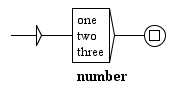
\includegraphics[width=13cm]{resources/img/fig5-14.png}
\caption{Copy-Paste of a multiple selection\label{copy-paste-multi-selection}}
\end{center}
\end{figure}

\bigskip
\noindent NOTE: You can paste a multiple selection into a different graph from
the one where you copied it from.

\bigskip
\index{Graph!deleting boxes}\index{Boxes!deleting}
\noindent In order to delete boxes, select them, delete the text that they
contain (\textit{i.e.} the text presented in the text field above the window)
and press the Enter key.

\bigskip
\noindent The initial and final states cannot be deleted.

\subsection{Transducers}
\label{Transducers}\index{Transducers}\index{\verb+/+}
A transducer is a graph in which outputs can be associated with boxes. To insert
an output, use the special character \verb+/+. All characters to the right of
it will be part of the output. Thus, the text \verb$one+two+three/number$ results in
a box like in figure~\ref{fig-exemple-transduction}.

\begin{figure}[h]
\begin{center}
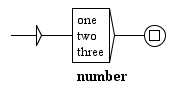
\includegraphics[width=4.5cm]{resources/img/fig5-15.png}
\caption{Example of a transducer\label{fig-exemple-transduction}}
\end{center}
\end{figure}

\noindent To create an empty box with an output consisting of \verb+number+, type \verb+<E>/number+ (example: the rightmost box in Fig.~\ref{fig-using-variable} is empty and has an output). The output associated with a box is represented in bold text below it.

\subsubsection{Weights}
\index{Weight}
You can assign integer weights to the boxes of a transducer.
Thus, when a sequence of tokens is matched by several paths with different outputs 
(ambiguous transducer\index{Ambiguous!transducer}\index{Transducer output!ambiguity}), only a path with the highest weight will produce an output. 
After a locate, this will affect the concordance, in which 
the matched sequences of words will appear only once with the appropriate output
(Figure~\ref{fig-weights-in-graphs}).

\begin{figure}[h!]
\begin{center}
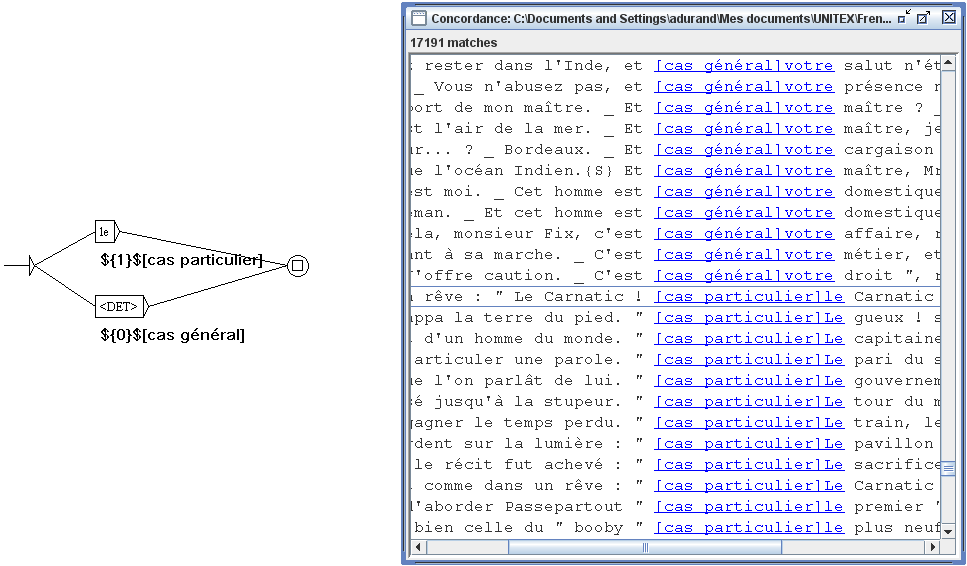
\includegraphics[width=14.5cm]{resources/img/fig5-15b.png}
\caption{weights in graphs \label{fig-weights-in-graphs}}
\end{center}
\end{figure}

\bigskip
\noindent In order to assign weight 1 to a box, insert \verb+${1}$+
in the output of the box, e.g. as in \verb+<E>/${1}$+.

\bigskip
\noindent The weight of a path is the latest weight found while traversing the path. A weight can be zero, but cannot be less than zero. A path with a weight (even zero) has higher precedence than a path without weight.

\bigskip
\noindent With weights, you can define a priority among paths that match the same sequence.
You cannot define a priority among embedded matching sequences (cf. section~\ref{section-search-configuration})
 or among overlapping matching sequences (cf. section~\ref{section-priority-leftmost-match}).
 
\bigskip
\noindent Weights are valid only within a graph, not in subgraphs or in calling graphs.

\subsection{Input Variables}
\label{section-using-variables}
\index{Graph!variables in a}\index{Variable!input}\index{\verb+$+}
\index{Transducer!with variables}

It is possible to select parts of a text sequence recognized by a grammar using input
variables. To associate an input variable \verb+var1+ with parts of a grammar, use the special
symbols \verb+$var1(+ and \verb+$var1)+ to define the beginning and the end of
the part to be stored. Create two boxes containing one \verb+$var1(+ and the second
\verb+$var1)+. These boxes must not contain anything but the variable name
preceded by \verb+$+ and followed by a parenthesis. Then link these boxes to the
zone of the grammar to be stored. The graph in
figure~\ref{fig-using-variable} recognises a sequence of digits before
\verb+dollar+ or \verb+dollars+. This sequence will be stored in a variable named
\verb+var1+.

\bigskip
\begin{figure}[h]
\begin{center}
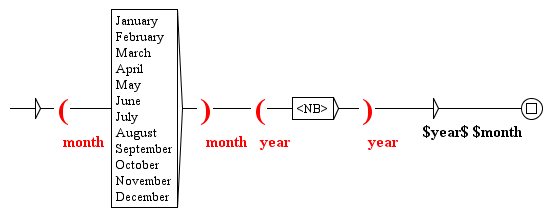
\includegraphics[width=13.5cm]{resources/img/fig5-16.png}
\caption{Using the input variable
\texttt{var1}\label{fig-using-variable}}
\end{center}
\end{figure}

\noindent Variable names may contain latin letters (without accents), upper or
lower case, numbers, or the \verb+_+ (underscore)
character.\index{\verb+_+}\index{Variable!names} Unitex distinguishes
between uppercase and lowercase characters.
\index{Underscore}

\bigskip
\noindent Once a variable is defined, you can use it in transducer outputs by
surrounding its name with \verb+$+.\index{\verb+$+} The grammar in
figure~\ref{fig-date-grammar} recognizes a date formed by a month and a
year, and produces the same date as an output, but in the order year-month.

\bigskip
\begin{figure}[h]
\begin{center}
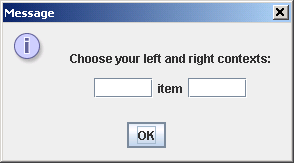
\includegraphics[width=14.5cm]{resources/img/fig5-17.png}
\caption{Inverting month and year in a date\label{fig-date-grammar}}
\end{center}
\end{figure}

\noindent If you want to use the character \verb+$+ in the output of a box, you
have to double it, as shown on figure~\ref{fig-using-variable}.

\bigskip
\noindent When a box redefines a variable that had already been defined,
\index{Variable!redefine} the new value overrides the previous one.
Thus, if the variable is defined in a loop,
the value of the variable just after the loop depends on the last iteration of the loop.

\bigskip
\noindent By default, \verb+Locate+ and \verb+LocateTfst+ 
consider that variables that have not been defined are empty.
\index{Variable!undefined}You can
modify this behavior as shown in section \ref{section-advanced-search-options}.
Moreover, it is possible to test whether a variable has been defined or not, as
shown in section \ref{section-variables}.

\subsection{Copying lists}
\index{Copying lists}
\index{Copy}\index{Paste}

It can be practical to perform a copy-paste operation on a list of words or
expressions from a text editor to a box in a graph. In order to avoid having to
copy every term manually, Unitex provides a mean to copy lists. To use this,
select the list in your text editor and copy it using <Ctrl+C> or the copy
function integrated in your editor. Then create a box in your graph, and press
<Ctrl+V> or use the "Paste" command in the "Edit" menu to paste it into the box.
A window as in Figure~\ref{fig-setting-contexts-for-multiple-copy}
opens:

\bigskip
\begin{figure}[h]
\begin{center}
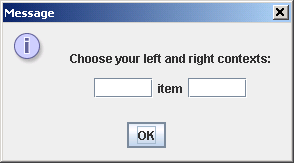
\includegraphics[width=7cm]{resources/img/fig5-18.png}
\caption{Selecting a context for copying a list\label{fig-setting-contexts-for-multiple-copy}}
\end{center}
\end{figure}
\index{Contexts!copy of a list}

\noindent This window allows you to define the left and right contexts that will
automatically be used for each term of the list. By default, these contexts are
empty. If you use the contexts  \verb+<+ and \verb+.V>+ with the following list:

\bigskip
\textit{eat}

\textit{sleep}

\textit{drink}

\textit{play}

\textit{read}

\bigskip
\noindent you will get the box in figure~\ref{fig-multiple-copy}:

\bigskip
\begin{figure}[h]
\begin{center}
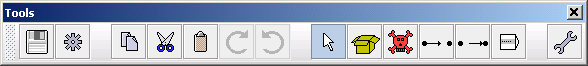
\includegraphics[width=6.7cm]{resources/img/fig5-19.png}
\caption{Box resulting from copying a list and applying contexts\label{fig-multiple-copy}}
\end{center}
\end{figure}

\subsection{Special Symbols}
\index{Symbols!special}
\noindent The Unitex graph editor interprets the following symbol in a special manner:

\bigskip
\verb," + : / < > # \,

\bigskip
\noindent Table~\ref{tab-special-symbols} summarizes the meaning of
these symbols for Unitex, as well as the ways to recognize these characters in texts.

\bigskip
\index{Meta-characters}
\begin{table}[h]
\begin{center}
\begin{tabular}{|c|p{9cm}|c|}
\hline
\texttt{Caracter} & \texttt{Meaning} & \texttt{Escape}
\\
\hline \verb$"$ & quotation marks mark sequences that must not be interpreted by
Unitex, and whose case must be taken verbatim & \verb$\"$
\\
\hline
\verb$+$ & \verb$+$ separates different lines within the boxes& \verb$"+"$
\\
\hline
\verb$:$ & \verb$:$ introduces a call to a subgraph& \verb$":"$ or \verb$\:$
\\
\hline
\verb$/$ & \verb$/$ indicates the start of a transduction within a box& \verb$\/$
\\
\hline
\verb$<$ & \verb$<$ indicates the start of a pattern or a meta & \verb$"<"$ or \verb$\<$
\\
\hline
\verb$>$ & \verb$>$ indicates the end of a pattern or a meta& \verb$">"$ or \verb$\>$
\\
\hline
\verb$#$ & \verb$#$ prohibits the presence of a space& \verb$"#"$
\\
\hline
\verb$\$ & \verb$\$ escapes most of the special characters & \verb$\\$
\\
\hline
\end{tabular}
\caption{Encoding of special characters in the graph
editor\label{tab-special-symbols}}
\end{center}
\end{table}

\subsection{Toolbar Commands}
\index{Toolbar}
\label{toolbar-commands}

The toolbar above a graph contains shortcuts for certain commands
and allows you to manipulate boxes of a graph by using some "tools". This
toolbar may be moved by clicking on the "rough" zone. It may also be dissociated
from the graph and appear in an separate window (see
figure~\ref{fig-toolbar}). In this case, closing this window puts
the toolbar back at its initial position. Each graph has its own toolbar.

\begin{figure}[!ht]
\begin{center}
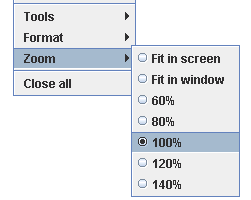
\includegraphics[width=15.6cm]{resources/img/fig5-20.png}
\caption{Toolbar\label{fig-toolbar}}
\end{center}
\end{figure}

%\bigskip
\medskip
\index{Copy}\index{Cut}\index{Paste}
\noindent The first two icons are shortcuts for saving and compiling the graph.
The following five correspond to the Copy, Cut, Paste, Redo and Undo operations. 

\bigskip
\noindent The following six icons correspond to edit commands for boxes. The first
one, a white arrow, corresponds to the boxes' normal edit mode. The next 5 icons
correspond to specific tools. In order to use a tool, click on the
corresponding icon: the mouse cursor changes its form and mouse clicks are then
interpreted in a particular fashion. What follows is a description of these
tools, from left to right:

\begin{itemize}
  \item creating boxes: creates a box at the empty place where the mouse was clicked;
  \item deleting boxes: deletes the box that you click on;
  \item connect boxes to another box: using this utility you select one or
  more boxes and connect it or them to another one. In contrast to the
  normal mode, the connections are inserted to the box where the mouse button
  was released on;
  \item connect boxes to another box in the opposite direction: this utility
  performs the same operation as the one described above, but connects the boxes
  to the one clicked on in opposite direction;
  \item open a sub-graph: opens a sub-graph when you click on a grey line within a box.
\end{itemize}
In order to change the cursor back to its normal form, the white arrow, right-click on the background of the graph:
then, mouse clicks will be interpreted in the normal way again.

\bigskip
\noindent The next icon (showing a wrench) is a shortcut to open the window with the graph display
options.
%%%%%%%%%%%%%%%%%%%%%%%%%%%%%%%%%%%%%%%%%
The following two icons allow you to view lists of graphs that are related to the current graph by a  "graph/subgraph" relation :
\begin{itemize}
\item The first displays a list of graphs called by the current graph
\item The second button shows the list of all the graphs calling the current graph as a subgraph.
\end{itemize}
The two green arrows button will refresh the current graph to load the latest version of the current graph. If any graph has its .grf file changed by any operation while displayed in a Unitex window, a window will pop up to warn you and invite you to refresh its window.

\bigskip
\noindent The balance button allows you to compare the current graph to another graph or another version of the same graph. This will display a new window (as in Figure~\ref{Graph-DIFF}) containing both graphs with colours pointing out the different types of changes between the two graphs: insertion, removal, moves of each state of the graph and change of the content of a state (respectively in green, red, purple and yellow).

\bigskip
\noindent 
\begin{figure}[!h]
\begin{center}
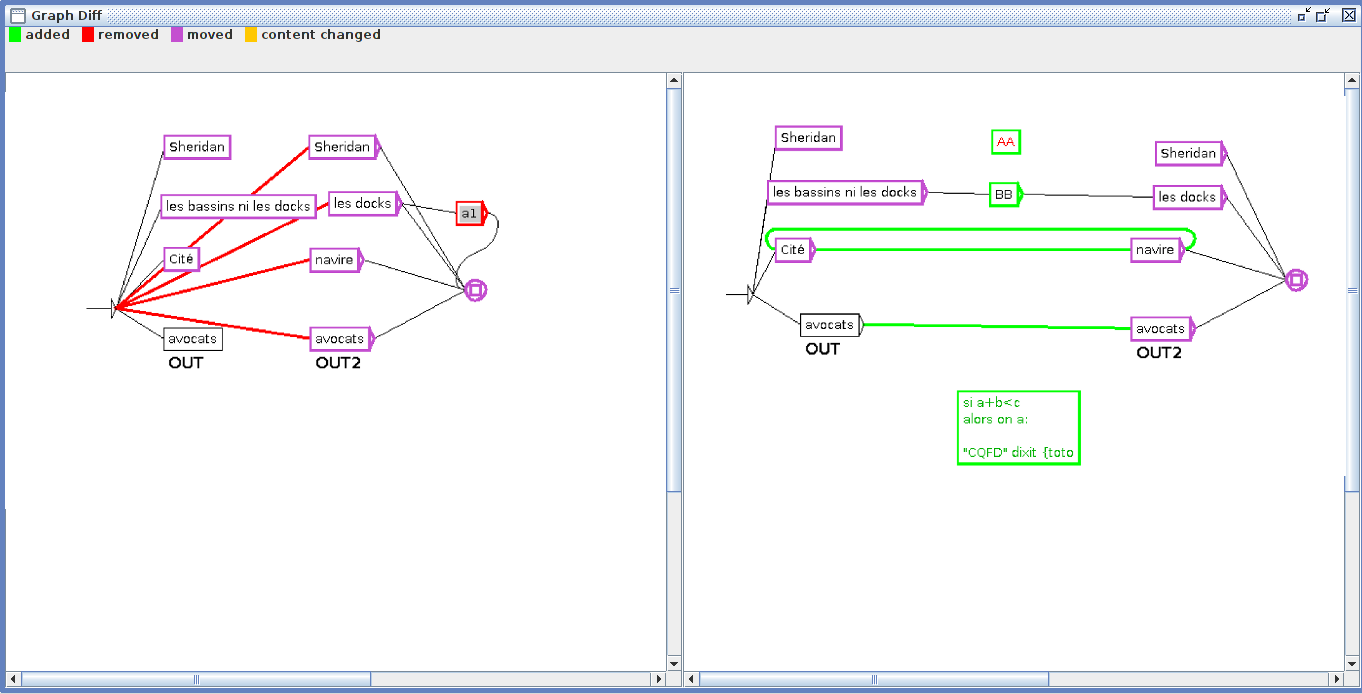
\includegraphics[width=15.6cm]{resources/img/DIFF.png}
\caption{DIFF\label{Graph-DIFF}}
\end{center}
\end{figure}
\bigskip
\noindent 

The last six buttons are shortcuts to use variables, morphological mode or insert contexts around one or several selected states. These buttons will be clickable only when one or several states are currently selected :
\begin{itemize}
\item \textcolor{red}{()}  : input variable	(see section~\ref{section-using-variables})
\item \textcolor{blue}{()} : output variable (see section~\ref{section-output-variables})
\item \textcolor{magenta}{<>}  : morphological mode (see section~\ref{section-morphological-mode})
\item \textcolor{green}{\$*} : left context (see section~\ref{section-contexts})
\item \textcolor{green}{\$[} : right context (see section~\ref{section-contexts})
\item \textcolor{green}{\$![} : negative right context (see section~\ref{section-contexts})
\end{itemize}

\bigskip
%\pagebreak
%%%%%%%%%%%%%%%%%%%%%%%%%%%%%%%%%%%%%%%%%
%%%%%%%%%%%%%%%%%%%%%%%%%%%%%%%%%%%%%%%%%
\section{Display options}
\index{Graph!display}

\subsection{Sorting the lines of a box}
\index{Sorting!lines of a box}\index{Boxes!sorting lines}
You can sort the content of a box by selecting it and clicking on "Sort Node
Label" in the "Tools" submenu of the "FSGraph" menu. This sort operation does
not use the \verb+SortTxt+ program. It uses a basic sort mechanism that sorts
the lines of the box according to the order of the characters in the Unicode
encoding.
\index{Unicode}

\begin{figure}[!h]
\begin{center}
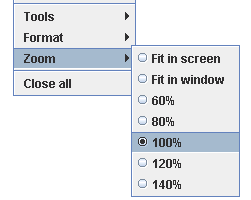
\includegraphics[width=6cm]{resources/img/fig5-21.png}
\caption{Zoom sub-menu}
\end{center}
\end{figure}
\subsection{Zoom}
\index{Zoom}\index{Graph!zoom}
The "Zoom" submenu allows you to choose the zoom scale that is applied to display the graph.
%\bigskip
\noindent The "Fit in screen" option stretches or shrinks the graph in order to fit it into the screen. The "Fit in window" option adjusts the graph so that it is displayed entirely in the window.

\clearpage
\subsection{Antialiasing}
\index{Antialiasing}\index{Graph!antialiasing}
Antialiasing is a shading effect that avoids pixelization
effects.\index{Pixellisation} You can activate this effect by clicking on
"Antialiasing..." in the "Format" sub-menu. Figure~\ref{fig-antialiasing}
shows one graph displayed normally (the graph on top) and with antialiasing (the
graph at the bottom).

\bigskip
\begin{figure}[!ht]
\begin{center}
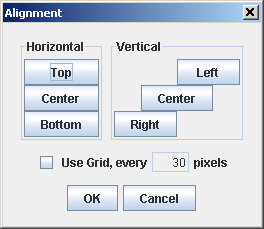
\includegraphics[width=13.5cm]{resources/img/fig5-22.png}
\caption{Antialiasing example\label{fig-antialiasing}}
\end{center}
\end{figure}

\noindent This effect slows Unitex down. We recommend  not to use it if your
machine is not powerful enough.

\clearpage 
\subsection{Box alignment}\index{Boxes!alignement}
\index{Box alignement}\index{Graph!box alignment}

In order to get nice-looking graphs, it is useful to align the boxes, both
horizontally and  vertically. To do this, select the boxes to align and click on
"Alignment..." in the "Format" sub-menu of the "FSGraph" menu or press <Ctrl+M>.
You will then see the window in Figure~\ref{fig-alignment-frame}.

\bigskip
\noindent The possibilities for horizontal alignment are:
\begin{itemize}
  \item Top: boxes are aligned with  the top-most box;
  \item Center: boxes are centered on the same axis;
  \item Bottom: boxes are aligned with the bottom-most box.
\end{itemize}

\begin{figure}[!h]
\begin{center}
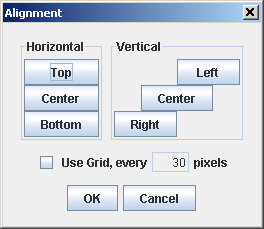
\includegraphics[width=6.6cm]{resources/img/fig5-23.png}
\caption{Alignment window\label{fig-alignment-frame}}
\end{center}
\end{figure}

\noindent The possibilities for vertical alignment are:
\begin{itemize}
  \item Left: boxes are aligned with the left-most box;
  \item Center: boxes are centered on the same axis;
  \item Right: boxes are aligned with the right-most box.
\end{itemize}

\bigskip
\noindent Figure~\ref{fig-vertical-left-alignment} shows an example
of alignment. The group of boxes to the right is (quite) a copy of the ones to the
left that was aligned.

\bigskip
\begin{figure}[!h]
\begin{center}
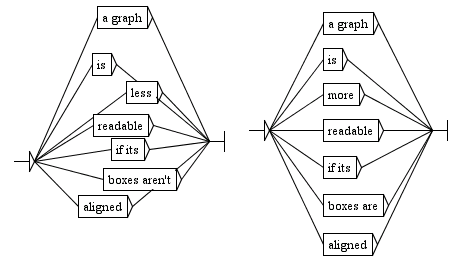
\includegraphics[width=11.5cm]{resources/img/fig5-24.png}
\caption{Example of box alignment\label{fig-vertical-left-alignment}}
\end{center}
\end{figure}

\bigskip
\noindent The option "Use Grid" in the alignment window shows a grid as the
background of the graph. This allows you to approximately align the
boxes.\index{Grid}

\bigskip
\begin{figure}[!h]
\begin{center}
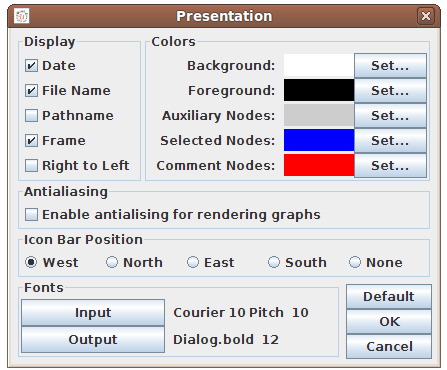
\includegraphics[width=15cm]{resources/img/fig5-25.png}
\caption{Example of using the grid}
\end{center}
\end{figure}

\subsection{Display options, fonts and colors}
\label{section-display-fonts-colors}
\index{Graph!display options, fonts and colors}\index{Options!configuration}
\index{Colors!configuration}
You can configure the display style of a graph by pressing <Ctrl+R> or by
clicking on "Presentation..." in the "Format" sub-menu of the "FSGraph" menu,
which opens the window as in
figure~\ref{fig-graph-display-configuration}.

\begin{figure}[!h]
\begin{center}
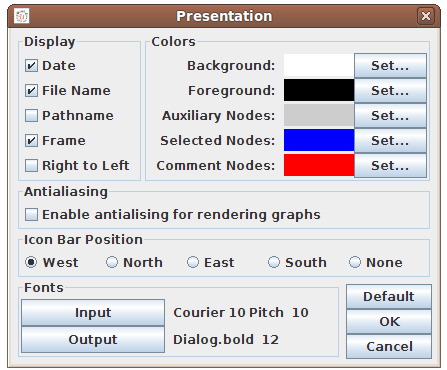
\includegraphics[width=9cm]{resources/img/fig5-26.png}
\caption{Configuring the display options of a graph\label{fig-graph-display-configuration}}
\end{center}
\end{figure}

\bigskip
\noindent The font parameters are:
\begin{itemize}
  \item Input: font used within the boxes and in the text area where the
  contents of the boxes is edited;
  
  \item Output: font used for the attached transducer outputs.\index{Transducer output}
\end{itemize}

\bigskip
\noindent The color parameters are:
\begin{itemize}
  \item Background: the background color;
  \item Foreground: the color used for the text and for the box display;
  \item Auxiliary Nodes: the color used for calls to sub-graphs;
  \item Selected Nodes: the color used for selected boxes;
  \item Comment Nodes: the color used for boxes that are not connected to others.
\end{itemize}

\bigskip
\noindent The other parameters are:
\begin{itemize}
  \item Date: display of the current date in the lower left corner of the graph;
  \item File Name: display of the graph name in the lower left corner of the graph;
  \item Pathname: display of the graph name along with its complete path in the
  lower left corner of the graph. This option only has an effect if the option
  "File Name" is selected;
  \item Frame: draw a frame around the graph;
  \item Right to Left: invert the reading direction of the graph (see an example
  in figure~\ref{fig-right-to-left-graph}).
\end{itemize}

\bigskip
\begin{figure}[!h]
\begin{center}
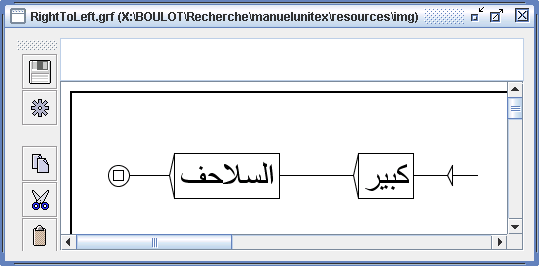
\includegraphics[width=14.5cm]{resources/img/fig5-27.png}
\caption{Graph with reading direction set to right to left\label{fig-right-to-left-graph}}
\end{center}
\end{figure}

\bigskip
\noindent You can reset the parameters to the default ones by clicking on
"Default". If you click on "OK", only the current graph will be modified. \index{Preferences} In
order to modify the preferences for a language as a default, click on
"Preferences..." in the "Info" menu and click on the "Graph configuration" button 
in the "Language \& Presentation" tab.


\section{Exporting graphs}
\label{exporting-graphs}
\subsection{Inserting a graph into a document}
\index{Graph!including into a document}\index{Including a graph into a document}
\index{PNG graph export}
In order to include a graph into a document, you have to convert it to an image.
To do this, export your graph to an image format: PNG, JPEG or SVG. Click on "Export as image" in the
"FSGraph" menu, and select a file format. You will get an image ready to be
inserted into a document, or to be edited with an image editor. You should
activate antialiasing for the graph that interests you (this is not obligatory
but results in a better image quality). Unlike JPEG, PNG uses lossless compression, so
PNG always look better than JPEG. Unlike PNG and JPEG, SVG format is not a bitmap format and
often look better. Using Inkscape, SVG file can be converted to EPS or PDF with command like:
\begin{verbatim}
Inkscape -z -E graph.eps graph.svg
\end{verbatim}
\begin{verbatim}
Inkscape -z -A graph.pdf graph.svg
\end{verbatim}

\bigskip
\noindent Another solution consists of making a screenshot:

\bigskip
\noindent On Windows:

\bigskip
\noindent Press "Print Screen" on your keyboard. This key should be next to the
F12 key. Start the \verb+Paint+ program in the Windows "Utilities" menu. Press
<Ctrl+V>. \verb+Paint+ will tell you that the image in the clipboard is too large
and asks if you want to enlarge the image. Click on "Yes". You can now edit the
screen image. Select the area that interests you. To do so, switch to the select
mode by clicking on the dashed rectangle symbol in the upper left corner of the
window. You can now select the area of the image using the mouse. When you have
selected the zone, press <Ctrl+C>. Your selection is now in the clipboard, you
can now just go to your document and press <Ctrl+V> to paste your image.

\bigskip
\noindent On Linux:

\bigskip
\noindent Take a screen capture (for example using the program \verb+xv+). Edit
your image at once using a graphic editor (for example \verb+TheGimp+), and paste
your image in your document in the same way as in Windows.

\newpage
\noindent\textbf{Vector graphics}
\index{SVG graph export}

\bigskip
\noindent If you prefer vector graphics, you can export your graph under the
SVG file format, which is editable with softwares like the Open Source
one Inkscape (\cite{Inkscape}). With this software, you can obtain PostScript
exports ready to use in pretty \LaTeX~documents.

\subsection{Printing a Graph}
\index{Printing!a graph}\index{Graph!printing}

You can print a graph by clicking on "Print..." in the "FSGraph" menu or by
pressing <Ctrl+P>.

\bigskip
\noindent WARNING: You should make sure that the page orientation parameter
(portrait or landscape) corresponds  to the orientation of your graph.

\bigskip
\noindent You can setup the printing preferences by clicking on "Page Setup"
in the "FSGraph" menu. You can also print all open graphs by clicking on "Print
All...".


